\documentclass[border=6pt]{standalone}
% Shared style for the methodology figures, after the block diagrams of
% "Attention Is All You Need": rounded blocks in soft colours with fine outlines,
% a grey container with a repetition count, and thin arrows.
\usepackage{libertinus}
\usepackage{amsmath}
\usepackage{xcolor}
\usepackage{tikz}
\usetikzlibrary{positioning,arrows.meta,calc,fit,backgrounds,shapes.geometric}

\definecolor{ink}{HTML}{1E2227}
\definecolor{muted}{HTML}{5C6670}
\definecolor{cRGB}{HTML}{2F6DB5}
\definecolor{cIR}{HTML}{C0622B}
\definecolor{cFuse}{HTML}{3B8B66}
\definecolor{cTime}{HTML}{7450A8}
\definecolor{cNeutral}{HTML}{66707B}
\definecolor{cData}{HTML}{8C6A2F}
\definecolor{cAlert}{HTML}{A8384A}
\definecolor{cHead}{HTML}{B08A2E}
\color{ink}

\tikzset{
  blk/.style   = {rounded corners=3pt, align=center, font=\small, inner xsep=6pt, inner ysep=4.5pt,
                  minimum height=0.8cm, line width=0.5pt, text=ink,
                  execute at begin node={\hyphenpenalty=10000}},
  vis/.style   = {blk, fill=cRGB!14, draw=cRGB!65},
  thr/.style   = {blk, fill=cIR!15, draw=cIR!65},
  fus/.style   = {blk, fill=cFuse!16, draw=cFuse!70},
  scn/.style   = {blk, fill=cTime!14, draw=cTime!65},
  neu/.style   = {blk, fill=cNeutral!10, draw=cNeutral!55},
  hed/.style   = {blk, fill=cHead!16, draw=cHead!70},
  dat/.style   = {blk, fill=cData!12, draw=cData!60},
  io/.style    = {align=center, font=\small, text=ink},
  op/.style    = {circle, draw=cNeutral!70, fill=white, line width=0.5pt, inner sep=0pt,
                  minimum size=5.2mm, font=\small},
  lab/.style   = {font=\footnotesize\itshape, text=muted, align=center},
  note/.style  = {font=\footnotesize, text=muted, align=left},
  ar/.style    = {-{Stealth[length=2.1mm,width=1.6mm]}, line width=0.55pt, draw=ink!75},
  dar/.style   = {ar, dash pattern=on 2.4pt off 1.6pt},
  gar/.style   = {ar, draw=cData, dash pattern=on 2.4pt off 1.6pt},
  box/.style   = {rounded corners=6pt, fill=cNeutral!5, draw=cNeutral!45, line width=0.5pt},
  over/.style  = {preaction={draw=white, line width=3.2pt, -}},
}

\begin{document}
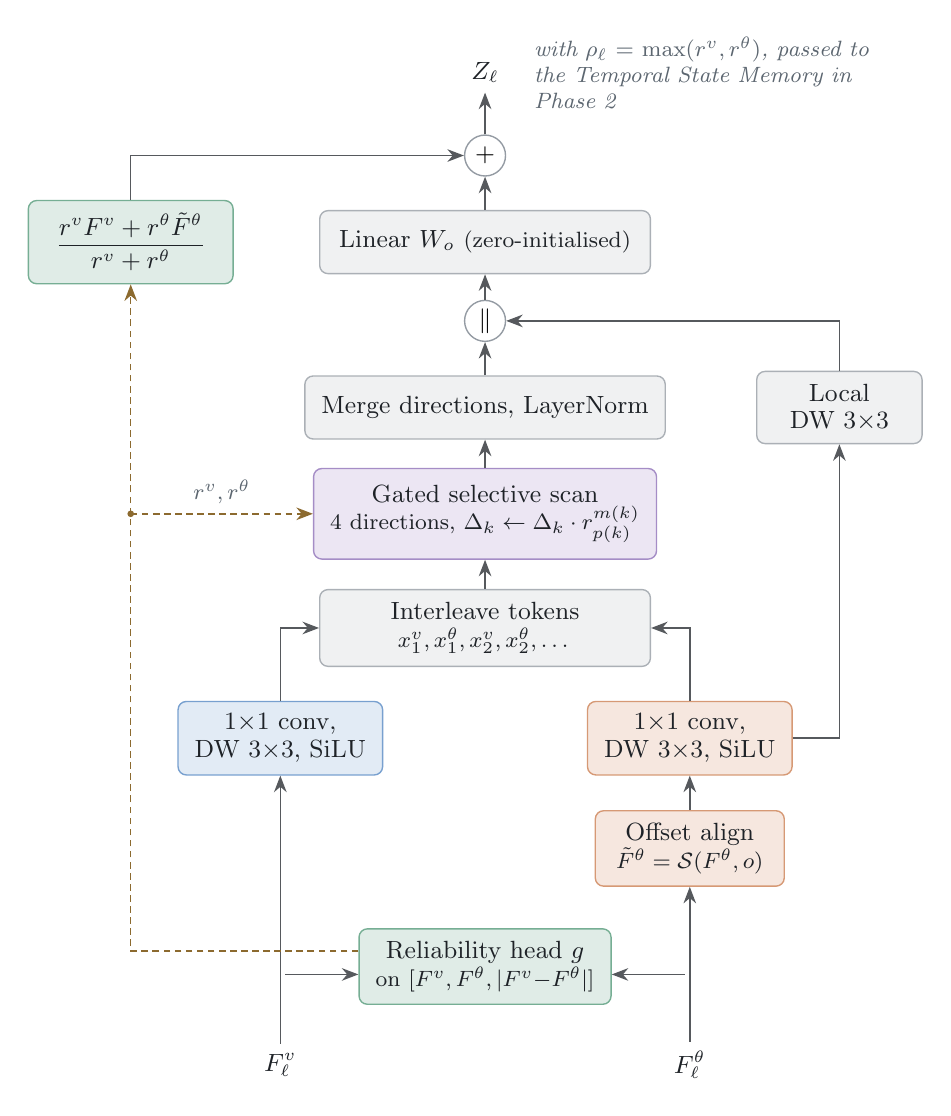
\begin{tikzpicture}
  % ---------------- inputs ----------------
  \node[io] (fv) at (0,0) {$F^{v}_\ell$};
  \node[io] (ft) at (5.2,0) {$F^{\theta}_\ell$};

  % reliability head between the inputs
  \node[fus, minimum width=2.9cm] (rel) at (2.6,1.25) {Reliability head $g$\\[-1pt] \footnotesize on $[F^v, F^\theta, |F^v{-}F^\theta|]$};
  \draw[ar] (fv) |- ($(rel.west)+(0,-0.1)$);
  \draw[ar] (ft) |- ($(rel.east)+(0,-0.1)$);

  % thermal alignment
  \node[thr, minimum width=2.4cm] (al) at (5.2,2.75) {Offset align\\[-1pt] \footnotesize $\tilde F^\theta = \mathcal{S}(F^\theta, o)$};
  \draw[ar, over] (ft) -- (al);

  % projections
  \node[vis, minimum width=2.4cm] (pv) at (0,4.15) {$1{\times}1$ conv,\\[-1pt] DW $3{\times}3$, SiLU};
  \node[thr, minimum width=2.4cm] (pt) at (5.2,4.15) {$1{\times}1$ conv,\\[-1pt] DW $3{\times}3$, SiLU};
  \draw[ar, over] (fv) -- (pv);
  \draw[ar] (al) -- (pt);

  % interleave and scan
  \node[neu, minimum width=4.2cm] (il) at (2.6,5.55) {Interleave tokens\\[-1pt] \footnotesize $x^v_1, x^\theta_1, x^v_2, x^\theta_2, \dots$};
  \draw[ar] (pv.north) |- (il.west);
  \draw[ar] (pt.north) |- (il.east);
  \node[scn, minimum width=4.2cm, minimum height=1.15cm] (sc) at (2.6,7.0)
       {Gated selective scan\\[-1pt] \footnotesize 4 directions, $\Delta_k \leftarrow \Delta_k \cdot r^{m(k)}_{p(k)}$};
  \draw[ar] (il) -- (sc);

  % merge and local branch
  \node[neu, minimum width=4.2cm] (mg) at (2.6,8.35) {Merge directions, LayerNorm};
  \draw[ar] (sc) -- (mg);
  \node[neu, minimum width=2.1cm] (lc) at (7.1,8.35) {Local\\[-1pt] DW $3{\times}3$};
  \draw[ar] (pt.east) -| (lc.south);
  \node[op] (cat) at (2.6,9.45) {$\Vert$};
  \draw[ar] (mg) -- (cat);
  \draw[ar] (lc.north) |- (cat.east);
  \node[neu, minimum width=4.2cm] (wo) at (2.6,10.45) {Linear $W_o$ \footnotesize(zero-initialised)};
  \draw[ar] (cat) -- (wo);

  % reliability-weighted residual
  \node[op] (add) at (2.6,11.55) {$+$};
  \draw[ar] (wo) -- (add);
  \node[fus, minimum width=2.6cm] (res) at (-1.9,10.45) {$\dfrac{r^v F^v + r^\theta \tilde F^\theta}{r^v + r^\theta}$};
  % one reliability signal feeds both the scan gate and the residual weights
  \draw[gar] ($(rel.west)+(0,0.2)$) -| (res.south);
  \draw[gar] (res.south |- sc.west) -- (sc.west) node[pos=0.5, lab, above] {$r^v, r^\theta$};
  \fill[cData] (res.south |- sc.west) circle (1.2pt);
  \draw[ar] (res.north) |- (add.west);
  \node[io] (z) at (2.6,12.6) {$Z_\ell$};
  \draw[ar] (add) -- (z);
  \node[lab, anchor=west, text width=4.4cm, align=left] (rho) at (3.1,12.6) {with $\rho_\ell=\max(r^v, r^\theta)$, passed to the Temporal State Memory in Phase 2};
\end{tikzpicture}
\end{document}
